\begin{theory}
 \chapter{Theory}
 \hyperlink{toc}{Return to TOC}
 \section{\label{ch2:sec0:level1}Preface}
  This chapter introduces a number of basic concepts related to the work outlined in the later chapters.
  I'll begin with a cursory overview of quantum chemistry which will provide a background for a more
  thorough discussion on symmetry adapted perturbation theory. Following this, I'll introduce some basics
  of molecular simulation to set the stage for a more in depth examination of the computational free energy
  methods used in my work.
  
  Sections \ref{ch2:sec1:level2}--\ref{ch2:sec1:level4} draw extensively from Refs. \cite{eschrig1996dft,ostlund}.
  This includes equation format and outline, but the text itself is original.
  
 \section{\label{ch2:sec1:level1}A primer on general electronic structure theory}
  \subsection{\label{ch2:sec1:level2}The Schr\"{o}dinger equation and multielectron wave functions}
   The principle goal of quantum chemistry is to find approximate solutions to the Schr\"{o}dinger equation.
   Below the equation is presented in its non-relativistic, time-independent form. This form is the most 
   commonly used in chemical literature.
 
   \begin{equation}\label{tise}
    \hat{H}\left|\phi\right> = \epsilon\left|\phi\right>
   \end{equation}
 
   In Eq. \ref{tise}, $\left|\phi\right>$ is the wave function of some system, $\hat{H}$ the Hamiltonian 
   operator which acts on the wave function, and $\epsilon$ the resulting energy eigenvalues. The 
   dimensionless Hamiltonian takes the form
 
   \begin{equation}\label{hamiltonian}
    \hat{H} = -\sum_{i=1}^{N} \frac{1}{2}\nabla_{i}^{2} -\sum_{a=1}^{M} \frac{1}{2M_{a}}\nabla_{a}^{2}
              -\sum_{i=1}^{N} \sum_{a=1}^{M} \frac{Z_{a}}{r_{ia}} +\sum_{i=1}^{N} \sum_{j>i}^{N} \frac{1}{r_{ij}}
              +\sum_{a=1}^{M} \sum_{b>a}^{M} \frac{Z_{a}Z_{b}}{R_{ab}}.
   \end{equation}
 
   Above, the first pair of terms denote the kinetic energy contributions made by the \emph{i}th electron and
   \emph{a}th nucleus through twice differentiation with respect to the particle coordinates. The middle term
   expresses the attraction between the \emph{i}th electron and \emph{a}th nucleus with Z$_{a}$ in reference to
   the atomic number of the nucleus. The final two terms represent the repulsion between electrons and nuclei,
   respectively. Here, r$_{ia}$, r$_{ij}$, and R$_{ab}$ are distances between the relevant particles and M$_{a}$ 
   the ratio of the mass of nucleus \emph{a} to the mass of an electron.
 
   Quantum chemists often simplify this problem by invoking the Born-Oppenheimer approximation which uncouples 
   electronic motions (fast) from nuclear motions (slow). In Eq. \ref{hamiltonian}, this amounts to dropping
   the second term on the right hand side while the final term becomes a constant. This reduced form is often
   termed the electronic Hamiltonian. Nuclear motions are handled by incorporating the electronic potential 
   (\emph{ab initio} molecular dynamics) or as a greatly simplified approximation of the electronic potential
   (classical molecular dynamics). In most applications, the nuclei are handled as point charges as more 
   computationally demanding procedures are required to include nuclear quantum effects. These effects can also
   be mimicked somewhat by simply increasing the temperature of a simulation. This trick is utilized in Chapter
   \ref{ch4:sec1:level1} to simulate the ethylene and propylene carbonate solvents in their liquid state.
 
   The electronic Hamiltonian we've reviewed so far has only considered the coordinates of the electron in space.
   For a complete description of an electron, however, we need to specify its spin as well. Thus, we have 
   $x=\{r,\omega\}$ such that the wave function of an N-electron system is 
   $\phi(x_{1}, x_{2}, \dots, x_{N})$ and is now a function of both spatial and spin coordinates. 
   The wave function of a many-electron system is simply the product of all the single-electron wave functions, 
   where $\phi(x_{1}, x_{2}, \dots, x_{N}) = \chi(x_{1})\chi(x_{2})\dots\chi(x_{N})$ and $\chi(x_{N})$ is the spin
   orbital of the \emph{N}th electron. We place an additional requirement on the electronic wave function that 
   it must be antisymmetric (change sign) upon exchange of the $x=\{r,\omega\}$ coordinate of any two electrons. 
   Antisymmetry forms the basis for all exchange and exchange-coupled terms in the symmetry adapted perturbation 
   theory and postulates that no two electrons can possess the same $x=\{r,\omega\}$ coordinates. A convenient 
   representation of the wave function of many-electron systems which satisfies antisymmetry is called a Slater 
   determinant. The Slater determinant takes the form of \emph{N}$\times$\emph{N}-matrix for an \emph{N}-electron
   system.
   
   In conventional modern electronic structure codes each of the single-electron products discussed in the previous paragraph 
   are represented using atom-centered orbitals. Each orbital comprises a radial and a spherical part. The solutions
   to the spherical part of the wave function derive from spherical harmonics, imparting shape and direction to the
   orbital. The radial part of the wave function generally assumes one of two forms: an exponential or a Gaussian.
   Though the exponential description is far more accurate, the Gaussian representation is considerably more 
   computationally efficient thanks to the Gaussian product theorem. A linear combination of one or more Gaussian 
   functions is used to approximate the exponential representation. The collection of atom-centered Gaussian orbitals
   used to represent the electronic structure of an atom is called a \emph{basis set}. Molecular systems are then
   modeled as a linear combination of these atomic orbitals,
   
   \begin{equation}\label{lcao}
    \phi_{i} = \sum_{\mu}^{n} c_{\mu i}\chi_{\mu}.
   \end{equation}   
   
   Above, $\phi_{i}$ is the resultant \emph{i}th molecular orbital from the sum over the \emph{n} atomic orbitals,
   $\chi_{\mu}$, each contributing $c_{\mu i}$ to the sum. The \emph{n} molecular orbitals represented as a 
   Slater determinant make up the wave function of many-electron, molecular systems used as input to Eq. \ref{tise}.
   In the next section we'll discuss the variational principle behind the Hartree-Fock method which minimizes the 
   total energy defined by the Hamiltonian in Eq. \ref{hamiltonian} by optimizing the expansion coefficients, 
   $c_{\mu i}$ in Eq. \ref{lcao} using only a single Slater determinant. The Hartree-Fock method forms the basis 
   of many of the more accurate electron correlation methods I'll discuss in brief as well.
   
  \subsection{\label{ch2:sec1:level3}Hartree-Fock and electron correlation methods}
  The Hartree-Fock approximation is a mean field theory which takes the simplifications addressed above a step
  further, with individual electrons modeled in the averaged field of the other electrons. The Hamiltonian
  becomes a summation over single-electron Fock operators which may be presented in the familiar eigenvalue 
  form of Eq. \ref{tise} as,
  
  \begin{equation}
   \emph{f}\left|\chi_{\alpha}\right> = \epsilon_{\alpha}\left|\chi_{\alpha}\right>.
  \end{equation}
  
  The Fock operator, \emph{f}, is convenient to separate into single-electron and two-electron terms as shown in
  Eq. \ref{focksep}.
  
  \begin{equation}\label{focksep} % leave as is
    \begin{split}
      \hat{H}_{0} = \sum_{i} \emph{f}_{i} &= \sum_{i} \left(\emph{h}_{i} + \nu^{HF}_{i}\right) \\
      \emph{h}_{i} &= -\frac{1}{2}\nabla_{i}^{2} - \sum_{a} \frac{Z_{a}}{r_{ia}} \quad\quad \textrm{where,} \quad r_{ia} 
      \equiv \left|r_{i}-r_{a}^{nuc}\right| \\
      \nu^{HF}_{i} &= \sum_{i<j} \left(J_{ij} - K_{ij}\right)
    \end{split}
  \end{equation}
  
  In Eq. \ref{focksep}, \emph{h} are the one-electron operators over kinetic energy and nuclear attraction 
  contributions. $\nu^{HF}$ denotes the two-electron Coulomb, \emph{J}$_{ij}$, and exchange integrals, 
  \emph{K}$_{ij}$. Solving the Hartree-Fock equations requires an iterative scheme to achieve self-consistency 
  (i.e., the orbitals found are the eigenfunctions of the Hartree-Fock Hamiltonian).
  
  Use of the mean field treatment of electron repulsion coupled with the single Slater determinant expansion
  of the wave function limits the accuracy of Hartree-Fock. van der Waals complexes where dispersion forces 
  play a significant role in the chemistry will be particularly poorly handled with this method. To improve
  upon the results of the Hartree-Fock method, there are a number of post-Hartree-Fock methodologies to consider
  for capturing the opposite-spin part of the correlation energy, $\epsilon_{corr} = E_{exact} - E_{HF}$. 
  Perturbation theory approaches such as M$\text{\o}$ller-Plesset perturbation theory treat the correlation energy as
  a perturbation of the Hartree-Fock Hamiltonian which tends to overcorrect for the missing energy. There are
  empirically tuned corrections such as spin-component scaling which generally muffle the same-spin two-electron
  integral contribution (same-spin correlation is already handled by Hartree-Fock). Configuration interaction
  and coupled cluster approaches make clever use of excitation operators to add additional excited determinants
  to the single Hartree-Fock reference determinant. These expansions are typically truncated to double, triple,
  or quadruple excitations to compensate for the high computational overhead associated with these methods.
  The perturbation or coupled cluster approaches are generally preferred as they are both size extensive and
  size consistent while truncated configuration interaction is not. With some dependence on the computational 
  resources at hand, coupled cluster and configuration interaction methods are typically limited to small 
  systems with no more than $\sim$ 100 electrons with a modest basis set. Though the use of a liberally 
  truncated virtual orbital space extends the size of systems accessible to treatment with a coupled cluster 
  approach. I made use of this technique in the CCSD(T)-level calculations in Chapter \ref{ch5:sec1:level1}. 
  By contrast, I was able to use an approximate form of M$\text{\o}$ller-Plesset perturbation theory with about 350
  electrons, also in Chapter \ref{ch5:sec1:level1}. However, for many systems such as that studied in Chapter
  \ref{ch4:sec1:level1}, a cheaper method for handling electron correlation may be required.
  
  \subsection{\label{ch2:sec1:level4}Density functional theory}
   \subsubsection{\label{ch2:sec1:level4:chasm1}Thomas-Fermi model of the electron gas}
   The precursor to density functional theory is the Thomas-Fermi model, which describes a uniformly distributed
   electron gas with electron density,
   
   \begin{equation}\label{thomasfermi}
       \rho(\vec{r}) = \frac{N}{V} = \frac{8\pi}{3h^{3}}p_{F}^{3},
   \end{equation}
  
  \noindent where $\rho(\vec{r})$ is the electron density, \emph{N} the particle number, \emph{V} the volume, 
  \emph{h} is Planck's constant, and \emph{p}$_{F}$ the Fermi momentum. The maximum allowed density is 2 
  electrons per \emph{h}$^{3}$. This theory is not suitable for describing bonding without a correction to the 
  kinetic energy which assumes the following form,
  
  \begin{equation}\label{weizsacker}
      T_{W}\left[\rho(\vec{r})\right] = \frac{\hslash^2}{8m} \int d^{3}r~ 
      \frac{\left|\nabla\rho(\vec{r})\right|^{2}}{\rho(\vec{r})}.
  \end{equation}
  
  \noindent Despite the deficiencies in the theory, Eq. \ref{weizsacker} highlights the fact that the properties
  of an electronic system can be expressed uniquely through the electron density itself. Hohenberg and Kohn built
  on this idea and developed an energy functional (\emph{E}$\left[\rho(\vec{r})\right]$) which is minimized for 
  the ground state electron density. They also proved that while the density is not known initially, it is possible 
  to variationally optimize it so as to minimize the functional. The solution also gives the ground state energy
  to within an additive constant. The energy functional is expanded below in Eq. \ref{hohenberg}.
  
  \begin{equation}\label{hohenberg}
      E\left[\rho(\vec{r})\right] = F\left[\rho(\vec{r})\right] + \int d^{3}r~ \rho(\vec{r})\nu_{ext}(\vec{r})
  \end{equation}
  
  The \emph{F}$\left[\rho(\vec{r})\right]$ functional is simply the kinetic and electron-electron repulsion terms
  from Eq. \ref{hamiltonian} (that's terms 1 and 4 on the rhs of the equation). $\nu_{ext}(\vec{r})$ is the 
  external potential created by the distribution of nuclei (term 3 in the Hamiltonian expression above). Recalling
  that under the Born-Oppenheimer approximation the kinetic energy contribution made by the nuclei is neglected
  and the nuclear-nuclear repulsion is constant, it is seen that the density functional theory provides an 
  alternative to Hartree-Fock theory to approximately solve the Schr\"{o}dinger equation using the electronic 
  Hamiltonian.
  
  Orbital-free or `pure' density functional theory seeks to solve Eq. \ref{hohenberg} through guessing the form
  of \emph{F}$\left[\rho(\vec{r})\right]$ and then optimizing the electron density from a trial density (i.e.,
  a guess) to minimize the energy functional. As with the Thomas-Fermi model, the kinetic energy functional is
  exceptionally difficult to characterize. The use of poor functionals produces considerable errors in the 
  properties of molecules compared to wave function theory. Nevertheless, Hohenberg and Kohn's theory for an 
  inhomogeneous electron gas laid the groundwork for the workhorse of modern day quantum chemistry which is 
  the Kohn-Sham formulation of density functional theory (KS-DFT).
  
  \subsubsection{\label{ch2:sec1:level4:chasm2}Kohn-Sham density functional theory}
  The Kohn-Sham equations build on the discussion above, improving the accuracy of the results through a clever
  trick which models \emph{N}-uncoupled electrons as if they were fully coupled. As a result, the Hamiltonian 
  reduces to a summation over \emph{N} single-electron Hamiltonians with approximate functionals to mimic proper
  electron-electron repulsion and electron correlation effects. This presents a similar eigenvalue problem to 
  that discussed in Chapter \ref{ch2:sec1:level3}. The benefit to this approach is that the kinetic energy of 
  non-interacting electrons is known \emph{exactly} in an orbital representation (KS-DFT uses basis sets and 
  produces orbitals just like Hartree-Fock) and the perturbation to fully interacting electrons is small compared 
  to the error in `pure' density functional methods. The energy functional in the Kohn-Sham approximation becomes,
  
  \begin{equation}\label{ksdft}
      E_{KS}\left[\rho\right] = E_{kin,KS}\left[\rho\right] + E_{Coul}\left[\rho\right] + E_{ext}\left[\rho\right]
      + \underbrace{\overbrace{\left(E_{kin}\left[\rho\right] - E_{kin,KS}\left[\rho\right]\right)}^{\lambda} + 
      E_{XC}\left[\rho\right]}_{E_{XC^{\prime}}\left[\rho\right]}
  \end{equation}
  
  \noindent where $\lambda$ is the uncoupled $\rightarrow$ coupled perturbation correction in the kinetic energy
  which is lumped in with the approximate exchange-correlation functional, E$_{XC^{\prime}}\left[\rho\right]$.
  
  The E$_{XC^{\prime}}\left[\rho\right]$ functional is not known exactly, just as the kinetic energy functional
  in Thomas-Fermi or Hohenberg-Kohn theories, but it turns out that even relatively simple forms work exceptionally
  well for estimating the exchange-correlation (XC) energy, see the \emph{local density approximation} (LDA). The 
  LDA method assumes the XC energy depends only on $\rho(r)$ without any dependence on the gradient of the density
  or the Kohn-Sham orbitals. This tends to lead to an over-estimation of the XC energy. Gradient-corrected XC
  functionals which include some contribution from $\nabla\rho(r)$ provide a substantial improvement over the LDA
  methods for molecular systems. Gradient-corrected functionals can be combined with some contribution from 
  \emph{exact} Hartree-Fock exchange to improve the results even further in so-called hybrid density functionals.
  Nowadays there are even double-hybrid density functionals which incorporate 2$^{nd}$ order M$\text{\o}$ller-Plesset 
  perturbation theory to add dispersion interactions without relying on empirically designed dispersion potentials
  (e.g., the D, D2, D3, and damped D3BJ corrections of Grimme or the exchange-hole dipole moment method of Johnson
  et al.\cite{becke2005exchange}). 
  
  In some cases it will be appropriate to add a further correction to condition the unphysical exponentially 
  decaying asymptotic behavior of the XC functionals which should go as 1/r at long range. These corrections differ
  for LDA/gradient-corrected functionals and the (double-)hybrid functionals. Hybrid functionals use range 
  separation similar to the Ewald summation method discussed in Chapter \ref{ch2:sec3:level4} to smoothly switch 
  to Hartree-Fock exchange. LDA and gradient-corrected functionals require a more sophisticated treatment discussed
  by Herbert et al.\cite{lao2014xsaptksd3}.
  
  \subsection{\label{ch2:sec1:level5}Wannier localization}
  Localization procedures are commonplace in quantum chemistry for concentrating charge density within atom-centered
  orbitals to speed up post-Hartree-Fock methods (e.g., local MP2\cite{lee2000closely}), be used in energy decomposition 
  analysis (e.g., the absolutely localized molecular orbitals method of Khaliullin et al.\cite{khaliullin2008almo}), or 
  discretize large clusters for decomposition into well-defined fragments which interact via a many-body expansion (e.g., 
  the fragment molecular orbital method\cite{kitaura1999fragment}). In many cases, researchers may be interested in
  simulating crystalline materials or solutions which make use of periodic 
  boundary conditions discussed in Chapter \ref{ch2:sec3:level3} to remove errors attributed to finite-size
  effects. At the \emph{ab initio} level, periodic codes make use of plane wave basis functions instead of
  conventional Gaussian ones or combine the technologies in a hybrid Gaussian plane wave method, which I use
  in Chapter \ref{ch4:sec1:level1}. The plane waves prevent us from simply being able to produce molecular
  orbitals as is commonplace in conventional electronic structure codes. This can be circumvented through
  the use of the Wannier localization which can condense even periodic plane wave basis functions into a set 
  of orthogonal atom-centered orbitals, each with -2\emph{e} charge where \emph{e} is the elementary charge.
  I use these orbitals to calculate the dipole moment of molecules of ethylene and propylene carbonate 
  molecules in the gas, condensed, and Li$^{+}$-solvating phases. These orbitals can also be used to calculate
  a number of other molecular or spectral properties. A more thorough discussion of the method can be found 
  here\cite{marzari2003mlwf}.
  
 \section{\label{ch2:sec2:level1}Symmetry adapted perturbation theory}
  The overall presentation and equation format is modeled after the Psi4 manual\cite{psi4sapt}, though the text 
  is original.
 
  The symmetry adapted perturbation theory (SAPT) is a technique used to partition interaction energies between
  fragments (i.e., between molecules but also now within 
  molecules\cite{parrish2015communication,pastorczak2015intramolecular}). The energies are partitioned
  into chemically interesting components: electrostatics, exchange-repulsion, induction, and dispersion. The
  induction contribution in SAPT is argued to be comprised of an intramolecular polarization component and a
  charge transfer component due to the exchange of fractional charge between molecules. Unlike other energy 
  decomposition schemes however, the polarization and charge transfer components of the interaction energy are
  not uniquely separable. A more thorough disucssion on this topic is presented in Chapter \ref{ch3:sec1:level1}.
  
  The SAPT Hamiltonian differs from the Hamiltonians we've examined previously. Instead of calculating the total
  energy of a molecule, we're only after the energy a system partitioned into fragments \emph{A} and \emph{B} is 
  lowered by due to their proximity to one another. This is handled through a perturbation theoretic expansion
  of the interaction energy in \emph{W}$_{A}$ + \emph{W}$_{B}$ and an interaction potential \emph{V} as shown in
  Eq. \ref{saptham}.
  
  \begin{equation}\label{saptham}
      \hat{H} = \emph{f}_{A} + \emph{f}_{B} + \left(W_{A} + W_{B}\right) + V
  \end{equation}
  
  In Eq. \ref{saptham}, the first two terms are the Fock operators we discussed in Chapter \ref{ch2:sec1:level1}.
  The next terms in parentheses, \emph{W}$_{A}$ + \emph{W}$_{B}$, are correlation operators. They are often 
  referred to as \emph{fluctuation potentials} for each of the monomers because the M$\text{\o}$ller-Plesset perturbation
  theory can also be interpreted as a measure of the deviation of the electron-electron repulsion from the mean
  (i.e., Hartree-Fock). These values are always the same since it makes no sense to treat one fragment at a higher
  perturbation order than the other. The interaction potential, \emph{V}, to first order decomposes into 
  electrostatic and exchange contributions and further into induction and dispersion components at second order.
  The \emph{symmetry adapted} part of the theory comes in the form of applying antisymmetrizers to project out 
  contributions made by Pauli-forbidden components of the interaction energy. These operators are applied to each 
  order in \emph{V} so, for example, the dispersion energy is equal to the sum of an attractive component and the 
  coupled exchange contribution. This is a separate energy from the 1$^{st}$-order exchange energy. An attractive
  feature of the SAPT formalism is that it is inherently free of basis set superposition error effects where 
  monomers `borrow' basis functions from neighboring atoms to approximate a more complete basis set. Below I'll 
  discuss some of the most common truncations of the theory.
  
  \subsection{\label{ch2:sec2:level2}SAPT0 and DFT-SAPT}
  SAPT0 is the lowest order truncation of the interaction energy. The `0' associated with the name of this truncation
  arises from each of the W$_{A}$ and W$_{B}$ perturbation operators set to 0\emph{th} order. The SAPT0 method 
  collects terms up to 2$^{nd}$ order in the interaction potential, however. The perturbation orders in the 
  expressions below are given as (\emph{V}\emph{W}).
  
  \begin{equation}\label{sapt0}
      E_{SAPT0} = E_{elst}^{(10)} + E_{exch}^{(10)} + E_{ind,resp}^{(20)} + E_{exch-ind,resp}^{(20)} + 
      E_{disp}^{(20)} + E_{exch-disp}^{(20)} + \delta_{HF}^{(2)}
  \end{equation}
  
  Above the `\emph{resp}' subscript denotes inclusion of orbital relaxation effects calculated through 
  coupled-perturbed Hartree-Fock. Where polarization effects are expected to be large, as is the case in the 
  ion/solvent cases explored in later chapters, the modeling of orbital response effects are necessary for 
  accurate energies. The final term in this series can be thought of as an \emph{ad hoc} correction to the 
  induction energy at low orders in \emph{V}.
  
  \begin{equation}\label{deltahf}
      \delta_{HF}^{(2)} = E_{int}^{HF} - (E_{elst}^{(10)} + E_{exch}^{(10)} + E_{ind,resp}^{(20)} + 
      E_{exch-ind,resp}^{(20)})
  \end{equation}
  
  In principle, the Hartree-Fock interaction energy accounts for electrostatic and induction components in the
  SAPT0 truncation to infinite order. It is also expected that the term is dominated by charge transfer 
  effects\cite{lande2015cdftct}. Taking the difference in the Hartree-Fock interaction energy and the 
  electrostatic and induction contributions recovered from SAPT0 is seen as an approximate way to add these 
  higher order effects in with no additional computational overhead.
  
  Density functional theory SAPT (or DFT-SAPT/SAPT(KS) for short) replaces the need for the correlation 
  operators in Hartree-Fock based SAPT and so is an attractive option for low cost and potentially highly
  accurate interaction energies. The expansion in \emph{V} is the same between the theories.
  
  \begin{equation}\label{dftsapt}
      E_{DFT-SAPT} = E_{elst}^{(1)} + E_{exch}^{(1)} + E_{ind,resp}^{(2)} + E_{exch-ind,resp}^{(2)} + 
      E_{disp}^{(2)} + E_{exch-disp}^{(2)}
  \end{equation}
  
  Assuming the \emph{exact} functional were known, the above expression would similarly be an \emph{exact}
  decomposition of the interaction energy within the SAPT formalism. It is critical to note that there is no
  singular way to carve up the interaction energy. Additionally, the poor asymptotic behavior in the Coulomb
  potential of modern density functionals must be corrected in order to improve the accuracy of the method 
  relative to the Hartree-Fock analogue. I make use of the Hartree-Fock reference SAPT scheme in Chapter
  \ref{ch3:sec1:level1} and a long-range corrected DFT-SAPT model in Chapter \ref{ch4:sec1:level1}. Dispersion
  interactions are treated explicitly in the former and via an empirical 
  model\cite{herbert2011xsapt1,herbert2012xsapt2,lao2014xsaptksd3} in the latter study.
  
  \subsection{\label{ch2:sec2:level3}SAPT2 and beyond}
  In this section I'll complete our discussion on the common truncations of the symmetry adapted perturbation
  theory, focusing now on the higher order terms. Higher orders of SAPT include 3$^{rd}$ order contributions
  in the interaction potential, \emph{V}, and non-zero orders in the correlation perturbation. For the following
  series of truncations to the SAPT interaction energy, the higher levels include all the terms for the previous
  levels and include correlation effects in electrostatic and induction terms (SAPT2), dispersion (SAPT2+),
  higher level electrostatic and dispersion effects (SAPT2+(3)), and full 3$^{rd}$ order terms in the exchange 
  and induction energies (SAPT2+3). This final truncation is typically the highest level offered by modern
  codes.
  
  \begin{equation}\label{sapt2}
   \begin{split}
      E_{SAPT2} = &E_{SAPT0} + E_{elst,resp}^{(12)} + E_{exch}^{(11)} + E_{exch}^{(12)} + ^{t}E_{ind}^{(22)} + \\
                  &^{t}E_{exch-ind}^{(22)}
   \end{split}
  \end{equation}
  
  \begin{equation}\label{sapt2p}
   \begin{split}
      E_{SAPT2+} = &E_{SAPT2} + E_{disp}^{(21)} + E_{disp}^{(22)}
   \end{split}
  \end{equation}
  
  \begin{equation}\label{sapt2p_3}
   \begin{split}
      E_{SAPT2+(3)} = &E_{SAPT2+} + E_{elst,resp}^{(13)} + E_{disp}^{(30)}
   \end{split}
  \end{equation}
  
  \begin{equation}\label{sapt2p3}
   \begin{split}
      E_{SAPT2+3} = &E_{SAPT2+(3)} + E_{ind,resp}^{(30)} + E_{exch-ind}^{(30)} + E_{exch-disp}^{(30)} + \\
                    &E_{ind-disp}^{(30)} + E_{exch-ind-disp}^{(30)} - \delta_{HF}^{(2)} + \delta_{HF}^{(3)}
   \end{split}
  \end{equation}  
  
  \begin{equation}\label{deltahf3}
      \delta_{HF}^{(3)} = \delta_{HF}^{(2)} - \left(E_{ind,resp}^{(30)} + E_{exch-ind}^{(30)}\right)
  \end{equation}
  
  Dispersion terms with non-zero correlation perturbation orders can be solved with coupled-cluster
  instead of M$\text{\o}$ller-Plesset \emph{t}-amplitudes. I make this substitution in later chapters involving
  SAPT2+ and higher calculations. I'm also truncating the correlated virtual orbital space by discarding
  natural orbitals below a defined threshold occupancy. This approximation, ideally, comes with negligible
  losses in accuracy. 
  
  The next sections will shift our focus from highly accurate but static descriptions of the electronic 
  structure in small ion/solvent clusters to modeling the motions of hundreds of particles for extended 
  lengths of time. To do this, I need to greatly simplify the physics and approximate the electronic energy 
  with efficient van der Waals potentials such as the Lennard-Jones, Buckingham, or Halgren functions.
  
 \section{\label{ch2:sec3:level1}A primer on molecular dynamics methods}
 Molecular dynamics (MD) is a computational technique for evaluating equilibrium and transport properties 
 of a many-body system\cite{smit}. MD simulation can be applied to a diverse range of chemical problems
 in the gas, condensed, or solid phase. The method is often used to compliment experimental results or 
 make predictions of behaviors that might ultimately be confirmed in subsequent experiments. However, the
 accuracy of these predictions hinges on a reasonable description of the interactions between molecules
 through some potential function, \emph{U}, typically modeled as a \emph{force field}. A force field applies
 a general formula for the interactions between atoms which become atom-specific through parameters tuned 
 for each atom, an atom in a specific functional group, or with a particular hybridization. In Chapter 
 \ref{ch4:sec1:level1} and other work not included in this thesis, I simulate with an \emph{ab initio} 
 potential directly. Much of the discussion below is applicable to these types of simulations as well.
 
 The scope of computer simulations has grown considerably since its infancy, with highly parallelized and
 efficient codes now handling up to millions of atoms. However, this still puts us many orders of magnitude 
 below the molar scale of Avogadro's number of particles, N$_{A}$. As such, molecular simulation \emph{in
 vacuo} operates well below the proper limit for simulating bulk liquids. This is because the forces acting 
 on surface molecules deviate from bulk behavior, introducing a set of finite-size artifacts into many 
 calculated properties. To circumvent this issue, we implement periodic boundary conditions to replicate the 
 finite system throughout space to remove the surface. Coulomb forces in periodic conditions require a unique 
 formula which splits the interactions into real space and reciprocal space. This technique is called Ewald
 summation. Modern MD codes typically use a more efficient solver than the one I will present in Chapter 
 \ref{ch2:sec3:level3}. Once we have solved for the potential and forces acting on the particles, we integrate
 Newton's equations of motion and solve for the new positions of all of the particles. The updated positions 
 have all new properties compared to the previous configuration -- and sometimes we wish to exert some level 
 of control over some of those properties to facilitate comparison to experiment. In this section, we'll 
 explore some of the tools behind the molecular dynamics method.
 
 The format of equations and general outline are modeled after Refs. \cite{tildesley,smit}. The wording is otherwise 
 original, as is the image.

 
  \subsection{\label{ch2:sec3:level2}Force fields and the potential energy function}
  At the heart of all classical simulations is the force field. The force field is two parts: (1) the potential
  energy function, \emph{U}, and (2) the optimized parameters used to represent a specific atom in the potential.
  The potential is an attempt to condense the Schr\"{o}dinger equation (Eq. \ref{tise}) to a more manageable
  level which can trace the dynamics of thousands of atoms across millions of individual force evaluations. 
  It is commonly expressed as a sum of a system's bonded and non-bonded contributions, with bonds, angles, and
  torsions modeled as harmonic springs (or periodic functions) with the stiffness controlled via a spring 
  constant as in Eq. \ref{gaff}.
  
  \begin{equation}\label{gaff}
   \begin{split}
      U = U^{bnd} + U^{nb} = &\sum_{bonds} k_{r}\left(r - r_{0}\right)^{2} + 
          \sum_{angles} k_{\theta}\left(\theta - \theta_{0}\right)^{2} + \\
          &\sum_{torsions} k_{\phi}\left(1 + cos\left(n_{\phi}\theta - \theta_{0}\right)\right) + \\
          &\sum_{Urey} k_{u}\left(u - u_{0}\right)^{2} + \\
          &\sum_{i\neq j} \frac{q_{i}q_{j}}{r_{ij}} + 
           \sum_{i\neq j} 4\varepsilon_{ij}\left(\left(\frac{\sigma_{ij}}{r_{ij}}\right)^{12} 
          - \left(\frac{\sigma_{ij}}{r_{ij}}\right)^{6}\right)
   \end{split}
  \end{equation}
  
  For some force fields, the torsion potential may be expressed with a harmonic potential similar to that 
  of the bonds, Urey-Bradley, and angle potentials. Not all force fields include the Urey-Bradley term which
  is sometimes called the (1,3) interaction where the indices refer to $\angle$123. In the periodic torsional
  potential, n$_{\phi}$ is the multiplicity. The last two terms in Eq. \ref{gaff} are the non-bonded terms,
  corresponding to the Coulomb and van der Waals (vdW) interactions, respectively. The vdW potential can take
  a number of different forms. Here, it is expressed as the Lennard-Jones potential where electron-electron
  repulsion is modeled as an \emph{r}$^{-12}$ potential instead of with an exponential as is the case with 
  the Buckingham potential. The \emph{r}$^{-6}$ dependent term is for dispersion interactions. In compliance
  with requirement (2) above, each atom is designated a partial charge, Lennard-Jones well-depth 
  $\varepsilon_{i}$, and radius $\sigma_{i}$. Mixing rules are used to generate the $\varepsilon_{ij}$ and
  $\sigma_{ij}$ terms specific to each atom/atom interacting pair. Another common exponent pair here is 14-7, 
  the buffered Halgren potential which I use with the AMOEBA polarizable force field in Chapter 
  \ref{ch5:sec1:level1}; additional sources on this force field can be found here\cite{laury2015revised}. 
  
  Partial charges (\emph{q}$_{i}$) are fit to reproduce the electrostatic potential of the atom or molecule at the
  Hartree-Fock, density functional, or M$\text{\o}$ller-Plesset perturbation level of theory. $\varepsilon_{i}$ and
  $\sigma_{i}$ for solvents are tuned to reproduce a plethora of macroscopic, mechanical, or solvation properties
  against experiment for the `pure' solvents. This causes issues when trying to model ion solvation in energy
  storage solvents which haven't seen as much attention from the community as has water. These parameters also
  tend to collect a lot of artificial contributions from sources that are not fully understood (see, for example,
  the surface potential of water). I show in Chapter \ref{ch6:sec1:level1} how this practice is troublesome.
  
  \subsection{\label{ch2:sec3:level3}Periodic boundary conditions}
  As described above, periodic boundary conditions are often used in simulations to remove non-negligible 
  surface effects which are present when the system is surrounded by a vacuum. A representation of a periodic
  cell is shown in Figure \ref{fig:pbc}. There are no hard walls to reflect molecules back into the box. 
  There are no longer spurious surface forces at the boundary as the mirrored exchange between the unit cell 
  and the image cells prevents the formation of a surface. 
  
  Applying periodic boundaries helps theorists to simulate the behavior of a much larger system with fewer
  particles and at greatly reduced computational cost. While abundantly useful in these purposes, there are a
  couple drawbacks to relying on periodic cells to mimic larger systems: (a) interactions between a particle and
  its image due to long-ranged (\emph{r}$^{-\nu}$) forces, where $\nu$ is less than the lattice dimensionality,
  (b) suppression of fluctuations with a wavelength longer than the lattice length, and (c) the presence of poorly
  understood, minor artifacts\cite{shirts2013simple}. The latter points (b, c) are not so critical for the work I've
  performed in this thesis, while the former (a) is a much more pressing concern. I'll discuss in the next 
  section the necessary corrections to the long-ranged Coulomb potential to remove unwanted image forces. 
  However, in the simulations I describe in Chapter \ref{ch6:sec1:level1}, I must consider the damping of 
  ion/dipole interactions via the solvent dielectric constant for which I have no correction. In this scenario,
  I want the lattice vector length to be at least as large as the Bjerrum length for a solvent, where Coulomb
  interactions between a particle and its periodic image become comparable to the thermal energy, k$_{B}$T, 
  with k$_{B}$ as Boltzmann's constant. This length scale varies with the inverse of the solvent dielectric 
  constant, $\lambda_{B} \propto \frac{1}{\epsilon}$. vdW forces on the other hand are short-ranged, requiring
  a lattice with a size of only $\approx$6$\sigma$ when using the Lennard-Jones potential.
  
  \newpage
  \begin{figure}
      \centering
      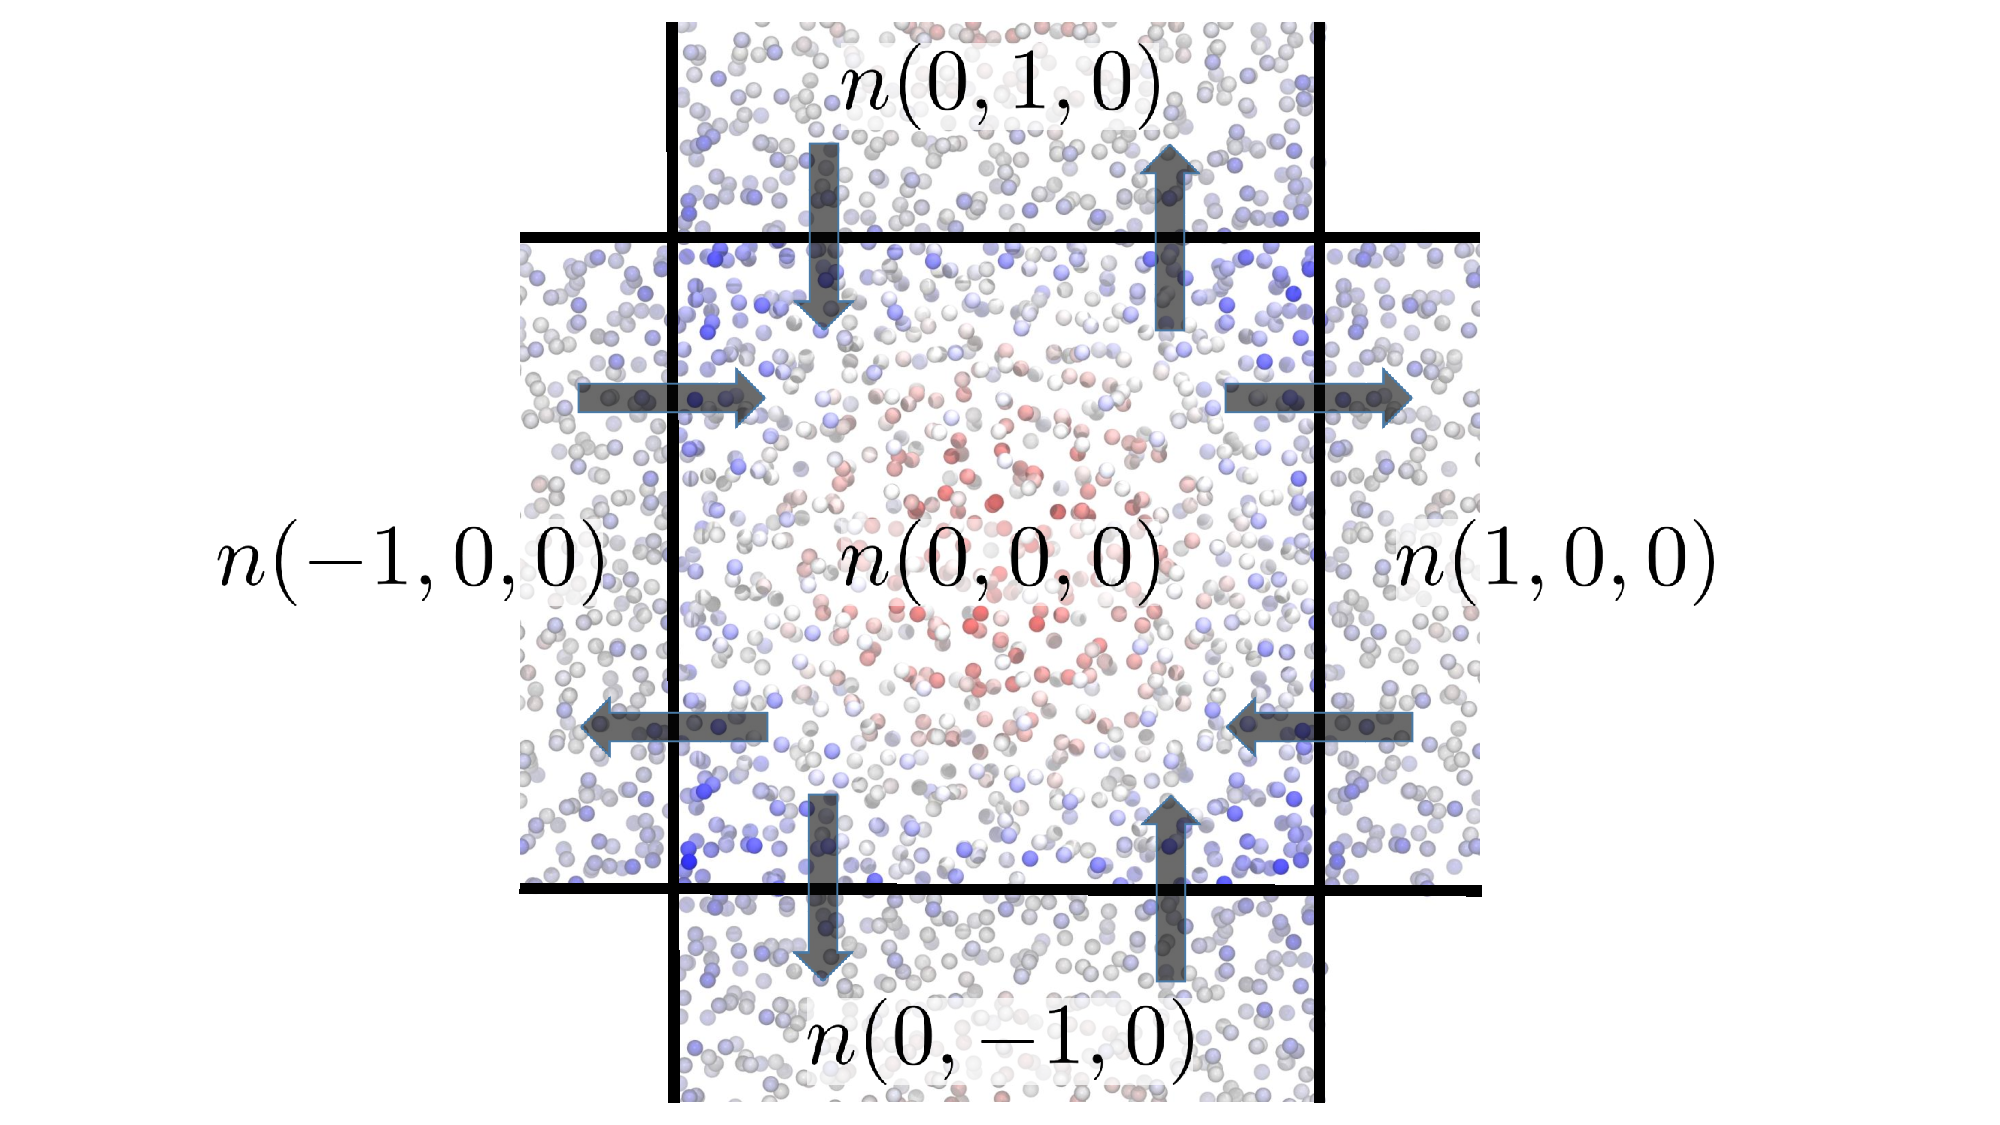
\includegraphics[width=0.98\linewidth]{images/pbc_example.pdf}
      \caption[Cartoon of a cubic periodic system]{Cartoon of a periodic cell with cubic lattice vectors of 
      length, \emph{L}. Particles are colored on a spectrum from red $\rightarrow$ white $\rightarrow$ blue
      by distance from the center of the cell. Each arrow is coupled with the one opposite it and indicates
      the direction of particle exchange between the unit cell \emph{n}(0,0,0) and the image cells 
      \emph{n}($\pm$x,$\pm$x,0). Because the motions are coupled between the unit and image cells, a particle
      exiting \emph{n}(0,0,0) and crossing into \emph{n}(1,0,0) is mirrored in \emph{n}(-1,0,0) as crossing 
      into \emph{n}(0,0,0) on the other side of the box.}
      \label{fig:pbc}
  \end{figure}
  
  \subsection{\label{ch2:sec3:level4}The Ewald summation}
  Assume we have a distribution of both positive and negative point charges scattered about a periodic and cubic
  cell of length, \emph{L}, and volume, \emph{L}$^{3}$. The total number of particles is \emph{N} and while we
  generally want \emph{N}/2 positive and \emph{N}/2 negative charges for charge neutrality, the discussion here
  will make no such demands. This makes sense especially since we are simulating \emph{infinitely dilute} single 
  ions where the unit cell is expected to take the same net charge as the ion inside. We want to calculate the
  Coulomb contribution to the potential energy of the system, which is expressed using a direct summation in Eq.
  \ref{directsum} (as in above sections, Gaussian units are assumed).
  
  \begin{equation}\label{directsum}
      U_{Coulomb} = \frac{1}{2} \sum_{i=1}^{N} \sum_{j=1}^{N} \sideset{}{'}\sum_{\textbf{n} \in \mathbb{R}} 
      \frac{q_{i}q_{j}}{\left|r_{ij} + \textbf{n}L\right|}
  \end{equation}
  
  The double sum runs over particle indices \emph{i} and \emph{j} up to the total number of particles \emph{N}
  over all cubic lattices where \textbf{n} = ($n_{x}$, $n_{y}$, $n_{z}$). $n_{x}$, $n_{y}$, and $n_{z}$ are
  integers which provide for the location of the lattice in 3D space, $\mathbb{R}$. The prime indicates that the 
  \textbf{n} = 0 sums should omit the \emph{i} = \emph{j} case so a particle does not interact with itself. In 
  principle the infinite sum of the series gives the true Coulomb energy in a lattice -- keyword, \emph{infinite}.
  To solve numerically, a finite set of lattice vectors are used under the assumption that as the distance from 
  the unit cell increases, the contribution to the potential will decrease as well. However, because the sum 
  converges very slowly a large cutoff must still be used to achieve sufficient accuracy. Combine this with a 
  hefty computational overhead of \textbf{\emph{O}}(\emph{N}$^{2}$) on the direct sum and it's easy to see why 
  a more efficient solver is desired. Ideally, an algorithm should scale linearly in cost with system size, 
  \textbf{\emph{O}}(\emph{N}). The most widely adopted algorithm in modern MD codes is the Ewald summation 
  \textbf{\emph{O}}(\emph{N}$^{\frac{3}{2}}$) or an even more efficient variant (i.e., particle mesh Ewald
  \textbf{\emph{O}}(\emph{N}log~\emph{N})).
  
  The Ewald summation splits the slowly converging series above into two components which can each be solved
  faster than the direct summation method. The series in 1/\emph{r} is usually split with the use of the error
  function $\erf$($\eta$r) and its complimentary form $\erfc$($\eta$r), where
  
  \begin{equation}
      \frac{1}{r} = \frac{erfc(\eta r)}{r} + \frac{erf(\eta r)}{r}.
  \end{equation}
  
  \noindent $\eta$ is a splitting parameter controlling the length scale and balance between the real space
  part, $\erfc$($\eta$r), and the reciprocal space part, $\erf$($\eta$r). In a cubic unit cell, $\eta$
  has an optimal value of 5.6/\emph{L} measured in \AA~with the real space part truncated to $\sim$10 \AA~and
  the reciprocal space part capturing the rest. The resulting formula takes the form,
  
  \begin{equation}\label{ewald}
   \begin{split}
      U_{Ewald} = &U_{real} + U_{recip} + U_{surf} + U_{self} + U_{net} \\
                = &\frac{1}{2} \sum_{i=1}^{N} \sum_{j=1}^{N} q_{i}q_{j} \left(\sideset{}{'}\sum_{\textbf{n} \in 
                \mathbb{R}} \frac{erfc(\eta\left|r_{ij} + \textbf{n}L\right|)}{\left|r_{ij} + \textbf{n}L\right|} + 
                \sum_{k \in \mathbb{K}, k \neq 0} \frac{4\pi}{L^3}\frac{e^{-\frac{k^2}{4\eta^2}}}{k^2}e^{-ik 
                \cdot r_{ij}}\right) + \\
                  & \frac{2\pi}{\left(2\epsilon^{\prime} + 1\right)L^3} \left(\sum_{i=1}^{N} q_{i}r_{i}\right)^2 + 
                  \frac{\zeta}{2L} \sum_{i}^{N} q_{i}^2 + \frac{\pi}{L^3\eta^2}Q^2,
   \end{split}
  \end{equation}
  
  \noindent where k=$\frac{2\pi}{L}\textbf{n}$ is the reciprocal space lattice vector, $\epsilon^{\prime}$ is the 
  dielectric of the surrounding medium, which is taken as $\infty$ in so-called `tin-foil' or conducting boundary
  conditions common to MD simulations and so vanishes, and Q$^{2}$ is the square of the net charge in the unit cell.
  The self-energy includes a constant $\zeta$ = -2.837297 for a cubic lattice. The corrections beyond the real and
  reciprocal space terms require little to no computational overhead and can sometimes be pre-computed and added in
  as a constant at each timestep, specifically when the volume is constrained. I use the more efficient 
  \textbf{\emph{O}}(\emph{N}$^{\frac{3}{2}}$) scaling algorithm in Chapter \ref{ch6:sec1:level1} for generating 
  trajectories but use a single sum version of the formula as presented in Eq. \ref{ewald} to compute the local 
  potential I described in Chapter \ref{ch1:sec4:level1}.
  
  \subsection{\label{ch2:sec3:level5}Equations of motion and time propagation}
  Once we have evaluated the potential energy of a configuration of particles, we calculate the force as the negative
  derivative of the potential with respect to the coordinate, $-\frac{\partial U}{\partial r}$. With forces in hand,
  we have a variety of mathematics to choose from to update the particle positions. One of the simplest and most 
  effective integrators is called the Verlet algorithm which is nearly universally available in modern MD codes.
  This method results from a Taylor series expansion in \emph{r} about time, \emph{t},
  
  \begin{equation}
      r(t+\delta t) \approx 2r(t) - r(t-\delta t) + \frac{f(t)}{m}\delta t^2,
  \end{equation}
  
  \noindent where $\delta$t is the length of the timestep and $\frac{f(t)}{m}$ is the acceleration on the particle
  for the current configuration. To compute the new location of a particle, various algorithms will require knowledge
  of one or more previous locations. The velocity of the particle can be computed from
  
  \begin{equation}
      v(t) = \frac{r(t+\delta t) - r(t-\delta T)}{2\delta t},
  \end{equation}

  \noindent which is accurate to order $\delta t^{2}$. From this, the kinetic energy and the system temperature can 
  be constructed. We'll see in the next section that this relation is important in monitoring the stability of a 
  simulation and/or conditioned so as to compare to an experiment under the same conditions.

  \subsection{\label{ch2:sec3:level6}Thermodynamic ensembles: controlling the variables}
  Thermodynamic ensembles are relations which establish a complete statistical knowledge of a system under certain
  conditions that are linked to macroscopic observables such as particle number, \emph{N}, temperature, \emph{T},
  energy, \emph{U}, or volume, \emph{V}. The natural ensemble for molecular dynamics simulations is the 
  \emph{microcanonical ensemble}, S(N,V,U), which is isolated from an external bath and the myriad parts merely 
  exchange the available energy to maximize the entropy throughout. This ensemble, in the limit of large systems,
  approximates the \emph{canonical ensemble} where average temperature is constant. Though in the \emph{canonical ensemble}, 
  this is accomplished through coupling to an external bath. 
  
  In both of these ensembles, the particle number and system volume are also fixed. The bath allows endo-/exothermic 
  processes to absorb/release excess energy through artificial modification of particle velocities. The \emph{canonical 
  ensemble} is widely used in molecular dynamics as precise control of the temperature is often necessary for studies of 
  protein folding, solvation thermodynamics, transport properties, etc. 
  
  The third most commonly used ensemble in molecular  dynamics is the \emph{isobaric-isothermal ensemble} where particle 
  number and temperature remain fixed as in the \emph{canonical ensemble} but the volume of the system is allowed to change
  to match a desired pressure. Motivations for controlling the pressure are similar to those for precise control on the 
  system temperature. Simulations incorporate barostats which scale the unit cell size in response to the virial pressure
  tensor which depends on the forces on the atoms. This ensemble is commonly used to relieve strain on the solvent after 
  adding large solutes such as proteins or other biomolecules to the unit cell and achieve a proper solvent density 
  especially at the cell edges. 
  
  Molecular dynamics relies on the ergodic principle to generate statistical averages of the behavior of molecular 
  systems through equivalence of averages in time to ensemble averages over all space. We must take great care with the 
  selection of an algorithm to constrain a particular property that it does not violate this condition, such as the original 
  Nos$\acute{e}$-Hoover thermostat. In the limit of large system size (\emph{N} $\rightarrow \infty$) the averages in 
  properties measured from each of the ensembles become identical. And so for the free energy work below, there is often
  very little difference between the averages computed in the (NVT) or (NpT) thermodynamic ensembles\cite{tlbbook}.
  
 \section{\label{ch2:sec4:level1}Free energy calculations using molecular dynamics}
 A knowledge of free energy and temperature derivatives is essential in advancing our understanding of a number of physical 
 phenomena including binding and equilibrium constants, rate constants of reactions, pH, pKa, activity coefficients 
 (solubilities), osmotic coefficients, surface tension, and partitioning behavior between phases (including phase transitions). 
 I will first present common methods for directly calculating free energies from molecular dynamics simulations. This will
 be followed by a thorough derivation and discussion of the quasichemical theory used in later chapters. The quasichemical 
 method partitions the solvation free energy through spatial conditioning. Taken together, the fragments add to the conventional
 solvation free energy but offer additional information not available to the other methods discussed here. The quasichemical 
 theory is particularly well-suited for the determination of single-ion solvation free energies because it is able to uniquely
 separate the local and distant solvation effects.
 
 The format of equations and general outline are modeled after Refs. \cite{smit,tlbbook}. The wording is otherwise original.
 
 \subsection{\label{ch2:sec4:level2}Free energy perturbation and thermodynamic integration}
 Free energy perturbation is one of the oldest and most successful methods for computing free energy differences between a
 reference state (A) and a target state (B). Recall that in the canonical ensemble, the Helmholtz free energy has the form,
 
 \begin{equation}\label{helmholtz}
     F(N,V,T) = -\frac{1}{\beta}\ln~Q_{NVT}.
 \end{equation}
 
 \noindent $\beta$ is the inverse temperature $\frac{1}{k_{B}T}$ and Q$_{NVT}$ is the canonical partition function. The partition 
 function can be split into coordinate and momentum space contributions, leading to an excess and an ideal contribution, 
 respectively.
 
 \begin{equation}\label{q_nvt}
  \begin{split}
      Q_{NVT} &= \frac{1}{N!}\frac{1}{h^{3N}}\int dp e^{-\beta\mathcal{K}} \int dq e^{-\beta\mathcal{V}} \\
              &= Q^{id}_{NVT}Q^{ex}_{NVT}
  \end{split}
 \end{equation}
 
 \noindent The ideal part is an analytical expression,
 
 \begin{equation}\label{q_id}
     Q^{id}_{NVT} = \frac{V^N}{N!\Lambda^{3N}}
 \end{equation}
 
 \noindent where the thermal de Broglie wavelength is $\Lambda = \sqrt{h^2/2\pi mk_{B}T}$. The excess part is
 
 \begin{equation}\label{q_ex}
     Q^{ex}_{NVT} = V^{-N}\int dr e^{-\beta\mathcal{V}(r)}.
 \end{equation}
 
 The free energy difference in the canonical ensemble, is
 
 \begin{equation}\label{fep}
     \Delta F(A\rightarrow B) = -\frac{1}{\beta}\ln\left<e^{-\beta\left(\mathcal{V}_{B}-\mathcal{V}_{A}\right)}\right>_{A}.
 \end{equation}
 
 \noindent $\mathcal{V}_{A}$ is the potential energy of the system in its reference state, and $\mathcal{V}_{B}$ is the energy
 of the system in the target state. The subscript indicates configurations are generated in the reference state. Angled brackets 
 indicate ensemble averaging. The single-perturbation result is only considered accurate if states A and B are very similar with
 strong overlap between the energy landscape outlined by their respective partition functions. If the mass does not change with 
 the perturbation, the ideal part vanishes. 
 
 Free energies between states with large perturbations (i.e., opposite charges, structural isomers, etc.) can be modeled as 
 incremental changes in the chemical properties of A to match B -- also known as `alchemical transformation.' The intermediate 
 states can be entirely fictitious so long as the i\emph{th} and (i+1)\emph{th} states are sufficiently similar. A coupling 
 parameter $\lambda$ is used to smoothly vary the A-state to B over (N-1) intervals. The coupling parameter can be chosen to 
 alter a single property at a time or several.
 
  \begin{equation}\label{alchemical}
     \Delta F(A\rightarrow B) = -\frac{1}{\beta} \sum_{i=1}^{N-1} \ln\left<e^{-\beta\left(\mathcal{V}_{\lambda_{i+1}}-\mathcal{V}_{\lambda_{i}}\right)}\right>_{\lambda_{i}}
 \end{equation}
 
 An alternative approach that also sees a great deal of use in the community is the thermodynamic integration method. This is 
 similar to the alchemical transformation approach described above in that we are attempting to connect two chemically 
 dissimilar endpoints using fictitious intermediates. However, instead of sampling the ensemble average in the difference of
 the energies between the (i+1)\emph{th} and i\emph{th} states, we sample the ensemble average of the derivative of the 
 potential with respect to the coupling parameter and then integrate,
 
 \begin{equation}\label{ti}
     \Delta F(A\rightarrow B) = \int_{0}^{1} d\lambda \left< \frac{\partial \mathcal{V}(\lambda)}{\partial \lambda}\right>_{\lambda}.
 \end{equation}
 
 As with free energy perturbation, numerous independent simulations at each $\lambda$ are required to assemble the final result. 
 These paths can be used to compute relative ion solvation free energies (e.g., K$^{+}$ to Na$^{+}$ or K$^{+}$ to Cl$^{-}$) and 
 absolute ion solvation free energies where the reference state is the ion uncoupled from the solvent. The ideal part of the free 
 energy is dropped here because it can be determined analytically, while the excess part is both the more interesting part and 
 far more difficult to compute. It is desirable to devise methods which require very few calculations for this excess part.
 
 \subsection{\label{ch2:sec4:level3}The potential distribution theorem}
 The potential distribution theorem of Widom \emph{sometimes called the particle insertion method} was developed to compute the 
 \emph{excess} chemical potential (i.e., partial molar free energy) of a solute in pure liquids or complex mixtures. In the 
 canonical ensemble, the excess chemical potential of a distinguished ion ($\alpha$) is
 
 \begin{equation}\label{mu}
     \mu^{ex}_{\alpha} = -\frac{1}{\beta}\ln\left<e^{-\beta\Delta\mathcal{V}}\right>_{0}; \quad\quad \textrm{where,} \quad \Delta\mathcal{V} = \mathcal{V}(N+\alpha)-\mathcal{V}(N)-\mathcal{V}(\alpha).
 \end{equation}
 
 \noindent $\Delta\mathcal{V}$ is the interaction energy between the ion and the solvent, with an ensemble average computed over
 configurations sampled with the ion uncoupled from the solvent (as indicated by the subscript `0'). The quantity is more 
 often expressed as
 
 \begin{equation}\label{bmu}
     \beta\mu^{ex}_{\alpha} = -\ln\left<e^{-\beta\Delta\mathcal{V}}\right>_{0}
 \end{equation}

 \noindent with an inverse form

 \begin{equation}\label{invbmu}
     \beta\mu^{ex}_{\alpha} = \ln\left<e^{\beta\Delta\mathcal{V}}\right>
 \end{equation} 
 
 \noindent where the sampling is now done over configurations which include the fully coupled ion/solvent interactions.
 Rearranging Eq. \ref{bmu} gives
 
 \begin{equation}\label{pmu}
     e^{-\beta\mu^{ex}_{\alpha}} = \left<e^{-\beta\Delta\mathcal{V}}\right>_{0} = \int d\varepsilon P_{\alpha}^{(0)}(\varepsilon)e^{-\beta\varepsilon}
 \end{equation}

 \noindent where $P_{\alpha}^{(0)}(\varepsilon) = \left<\delta\left(\varepsilon-\Delta\mathcal{V}\right)\right>_{0}$ is 
 a probability distribution of ion/solvent interaction energies from an uncoupled trajectory. Conversely, the distribution 
 from the fully coupled trajectory is $P_{\alpha}(\varepsilon) = 
 \left<\delta\left(\varepsilon-\Delta\mathcal{V}\right)\right>$. Using the law of averages we can relate these two 
 distributions through
 
 \begin{equation}\label{cross}
     P_{\alpha}(\varepsilon) = e^{-\beta\left(\varepsilon-\mu^{ex}_{\alpha}\right)}P_{\alpha}^{(0)}(\varepsilon).
 \end{equation}
 
 \noindent The crossing point of these distributions at some interaction energy $\varepsilon$ will yield the exact excess 
 chemical potential. If however, the distributions do not overlap, the method fails outright. The excess chemical potential
 can be assessed from one of the distributions as well, though the wings of these distributions are poorly, if ever, sampled
 over the course of a simulation making it difficult to integrate accurately. The quasichemical theory I discuss next addresses
 this by applying spatial conditioning to the interaction energy distributions. This removes the need to sample rare events 
 at the high- and low-energy tails of the distributions and yields Gaussian or nearly-Gaussian behavior in 
 $P_{\alpha}(\varepsilon)$. The conditioning is done using hard spheres with interaction energies computed only when all solvent
 is beyond a certain distance, or by adding an external potential into the simulation to push the solvent away. The latter is
 done gradually using thermodynamic integration.

 \subsection{\label{ch2:sec4:level4}Quasichemical theory}
 This section borrows equation format and outline from Refs. \cite{shi2013length,tlbbook}. The wording is otherwise
 original.
 
  \subsubsection{\label{ch2:sec4:level4:zone1}Hard sphere conditioning}
  Recall that the excess chemical potential of a monoatomic ion may be evaluated using the following expressions, derived 
  from the potential distribution theorem,

  \begin{equation}
   \begin{split}
    \beta\mu\sur{ex} &= -\mathrm{ln}\left<e^{-\beta\Delta\mathcal{V}}\right>\sous{0} \\
                     &=  \mathrm{ln}\left<e^{\beta\Delta\mathcal{V}}\right>,
    \label{eqn:pdt}
   \end{split}
  \end{equation}

  \noindent where $\beta = 1/k\sous{B}\mathrm{T}$ and $\Delta\mathcal{V}$ is the interaction energy between ion
  and solvent. Brackets indicate ensemble averaging. The subscript zero implies uncoupled ion/solvent motions
  during sampling and fully coupled ion/solvent interactions in the second case. In both cases, full 
  solvent/solvent interactions are in place. Inclusion of a hard-sphere cavity potential with radius, \emph{r}, 
  in the above expressions allows us to spatially separate contributions to the free energy,

  \begin{equation}
   \begin{split}
    \beta\mu\sur{ex} &= \mathrm{ln}\left<e^{-\beta\mathcal{V}\sous{HS}(r)}\right> - \mathrm{ln}\left<e^{-\beta\mathcal{V}\sous{HS}(r)}\right>\sous{0} - 
                        \mathrm{ln}\left<e^{-\beta\Delta\mathcal{V}}\right>\sous{\mathcal{V}\sous{HS}(r)} \\
                     &= \mathrm{ln}x\sous{0}(r) - \mathrm{ln}p\sous{0}(r) - \mathrm{ln}\left<e^{-\beta\Delta\mathcal{V}}\right>\sous{\mathcal{V}\sous{HS}(r)} \\
                     &= \mu\sursous{ex}{is}(r) + \mu\sursous{ex}{pk}(r) + \mu\sursous{ex}{os}(r).
    \label{eqn:hsqct}
   \end{split}
  \end{equation}

  Above, \emph{x}\sous{0} is the inner shell (is) term which is the probability of finding no solvent in the 
  excluded volume defined by $\mathcal{V}$\sous{HS} with full ion/solvent interactions, \emph{p}\sous{0} is 
  the packing (pk) term which is the probability of finding no solvent in this same cavity placed in pure 
  solvent, and the final term is the outer shell (os) or long-range term corresponding to the residual 
  interaction energy of the ion with solvent molecules beyond this excluded volume. A hard-sphere potential 
  suffices for small cavities typically around 0.3 nm or less, beyond which \emph{x}\sous{0} and 
  \emph{p}\sous{0} are generally poorly sampled in typical simulations. An external potential applied to the
  solvent is critical for reaching length scales far enough to see convergence in the interfacial potentials
  monitored as the mean-field electrostatic potential at the cavity's core.
  
  \subsubsection{\label{ch2:sec4:level4:zone2}Soft-core conditioning}
  I can reach any length scale by gradually introducing a soft-core M(\emph{r})-potential instead (Eq. \ref{eqn:scqct}).
  
  \begin{equation}
   \begin{aligned}
    \beta\mu\sur{ex} &= \mathrm{ln}\left<e^{-\beta M(r)}\right> - \mathrm{ln}\left<e^{-\beta M(r)}\right>\sous{0} - 
                        \mathrm{ln}\left<e^{-\beta\Delta\mathcal{V}}\right>\sous{M(r)} \\
                     &= \mathrm{ln}\left<e^{-\beta M(r)}\right> - \mathrm{ln}\left<e^{-\beta M(r)}\right>\sous{0} +
                        \mathrm{ln}\left<e^{\beta\Delta\mathcal{V}}\right>_{M(r)+\Delta\mathcal{V}}
    \label{eqn:scqct}
   \end{aligned}
  \end{equation}  
  
  In this framework, the packing and inner shell parts of the solvation free energy are captured by the work to dig
  a cavity in the bare solvent and around the ion, respectively. The inner shell portion is often referred to as the
  chemical part of the free energy as it's magnitude reflects the intensity of the interactions between the ion with 
  the retreating solvent. The thermodynamic integration procedure and M(\emph{r})-potential used in Chapter 
  \ref{ch6:sec1:level1} are the same as in a previous study\cite{shi2013length}. This arrangement requires two simulations
  for the outer shell contribution where ion/solvent interaction energy distributions are sampled from an uncoupled 
  and a separate coupled trajectory. The cavity radius, \emph{r}, should be tuned such that both distributions are
  accurately Gaussian. A mean-field approximation to $\mu$\sursous{ex}{os} can be obtained this 
  way\cite{hummer1996, hummer1998}, but as Shi and Beck demonstrated especially for anions, the fluctuation terms often
  do not match until reaching extreme length scales which can lead to inaccuracies\cite{shi2013length}. This behavior 
  has quite a bit to do with the similarities in the solvation shell between a neutral particle and one bearing 
  $\pm$q charge (e.g., orientation of solvent dipoles). I discuss more on this later in Chapter \ref{ch6:sec1:level1}.

  To work around this issue I invoke the midpoint-rule to generate an approximation to the long-range term from a 
  single simulation. Here the average interaction energy is sampled from a half-coupled trajectory where the ion's 
  charge is halved but all other interactions are unchanged. The approximation is accurate to second order in 
  perturbation theory and has proven remarkably reliable in previous free energy work\cite{beck2011lmft, shi2013length}.

\end{theory}
